\documentclass[english]{article}
\usepackage[T1]{fontenc}
\usepackage[utf8]{luainputenc}
\usepackage{geometry}
\usepackage[pdftex]{graphicx}
\geometry{verbose,tmargin=3cm,bmargin=3cm,lmargin=3cm,rmargin=3cm}
\usepackage{amssymb}
\usepackage{babel}
\begin{document}

\title{Software Engineering Coursework 1 - Othello}


\author{Rohan Mahtani \hspace{1cm} Varun Verma \hspace{1cm} Mihai Jiplea}

\maketitle

\section{Introduction}

The game of Othello (Reversi), is a two player strategy game involving
a square board and playing pieces that take the form of counters which
are white on one side and black on the other. Players take turns to
place pieces on the board, attempting to surround their opponent's
pieces. Any opposing pieces that are surrounded are flipped over and
converted from white to black, or vice versa. At the end of the game,
the winner is the player with more pieces of their colour on the board
(Summarized from specification).


\section{Design}


\subsection{Description}

There are five major packages: 


\subsubsection{Display: }
\begin{itemize}
\item Display interface: enables us to implement different visual representations. 
\item Includes a CommandLineDisplay class and a GUIDisplay class which both
implement the Display interface.
\end{itemize}

\subsubsection{Game:}
\begin{itemize}
\item Board class: Creates a board, which is a 2 dimensional array of Pieces.
At the start of the game, each array element of the board is a null
instance of Piece.
\item Colour enum: This enum contains the possible colours of the pieces.
Since it is a two player game, the elements of the enum Colour are
Black \& White, but this can easily be extended by adding additional
colours.
\item Game abstract class \& ReversiGame class: The ReversiGame class extends
the Game abstract class. Although the project's focus is creating
a Reversi game, the Game abstract class outlines methods that can
be used in a general game. Thus, if a Chess game was to be created,
it would be possible to extend the Game abstract class and reuse some
of the methods.
\end{itemize}

\subsubsection{Piece:}
\begin{itemize}
\item Piece abstract class and ReversiPiece class: The ReversiPiece class
extends the Piece abstract class. The relationship between these two
classes is very similar to the relationship between the Game and ReversiGame
classes. The ReversiPiece represents each piece on the board. The
colour of the piece is stored, while there is a flip method which
changes the colour of the piece.
\end{itemize}

\subsubsection{Player:}
\begin{itemize}
\item Player abstract class, RandomAIPlayer, and HumanPlayer class: The
HumanPlayer and RandomAIPlayer classes extend the Player abstract
class. This follows the same style as the Game \& Piece classes. The
Player's attributes are its name and its piece's colour. Both subclasses
have different implementations for the getMove method. The HumanPlayer
class gets a move by reading the user's input through a Scanner, while
the AI Player generates a move.
\end{itemize}

\subsubsection{Tests}
\begin{itemize}
\item There are four JUnit test classes, which test individual components
of the game. The following components are tested: Board, Human Player,
Reversi Game, and Piece.
\end{itemize}

\subsection{UML}

The UML (shown below) describes the overall implementation of the
game. \\
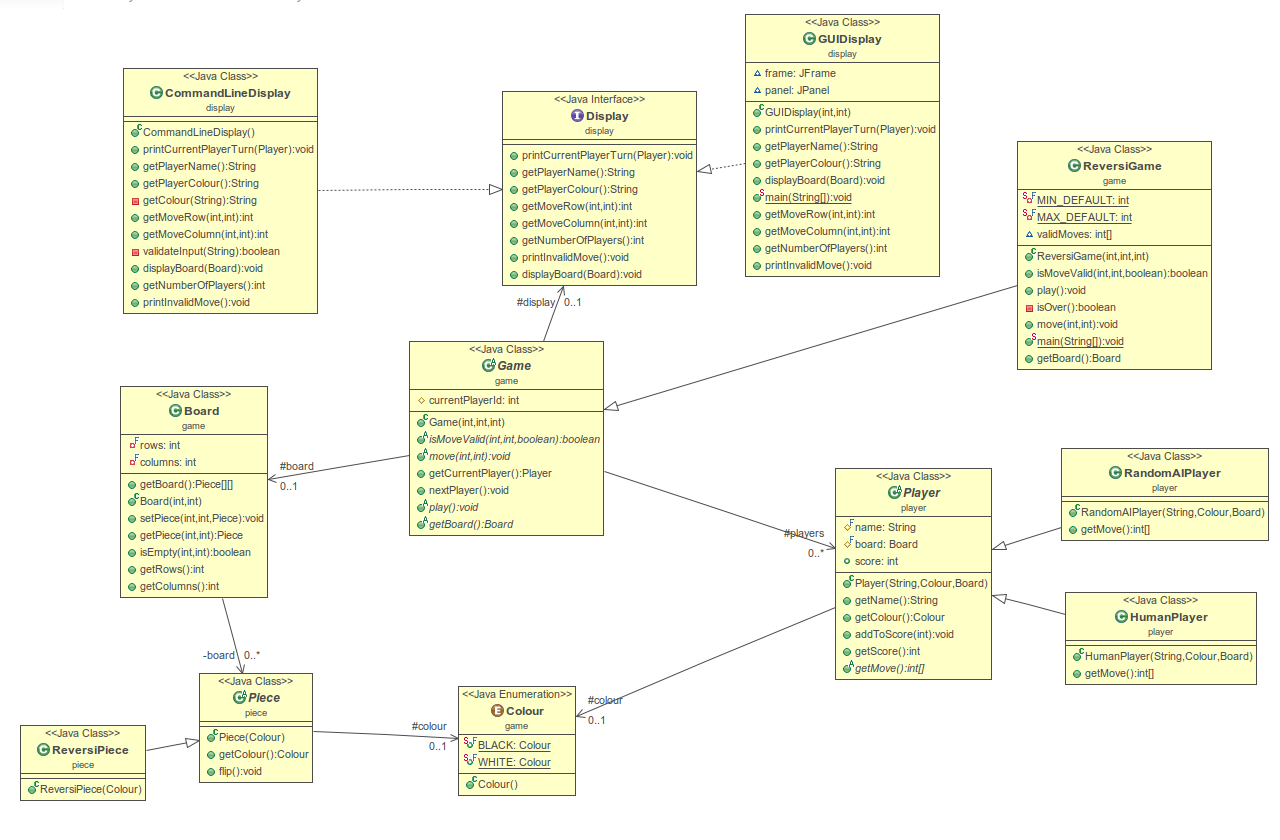
\includegraphics[width=7in]{UML}

\subsection{Design Decisions}
\subsubsection{Interfaces:}
\begin{itemize}
\item Used in: Display interface - GUI and Command Line displays implement
the display interface
\item The displays can be easily switched between a command line or a GUI
display, depending on what the user prefers, without changing the
actual implementation of the game. This also enables the use of polymorphism.
The advantages of polymorphism in relation to the Reversi code are
listed and explained in the section 2.3.4. 
\end{itemize}

\subsubsection{Abstract classes}
\begin{itemize}
\item Used in : Game, Player, Piece class
\item An example of this design decision is the Game abstract class and
a ReversiGame class which extends the Game. The Game class has methods
that deal with the current player and the player's turn and the ReversiGame
class inherits these methods. This allows us to implement multiple
two player games and reuse the same Game class, minimizing duplication.
The ReversiGame class further implements methods like checking if
a move is valid, which varies from game to game.
\item Player is an abstract class, and the reason for this implementation
is so that different types of players can be added easily. One example
is the simple AI Player, where the only method that needs to be changed
is the getMove method, which decides how a move would be selected.
For the Human Player class, the getMove method consists of getting
the user's input. An extension that we could implement and easily
integrate into our design is adding different difficulty levels for
the Computer Player - again, only the getMove method must be changed,
and different algorithms can be used in each getMove method.
\item Piece is an abstract class as well. If different games were to be
implemented with the same design, different types of pieces may be
needed. The abstract class allows a much easier implementation of
this.
\end{itemize}

\subsubsection{Model-View-Controller}

The design follows the Model-View-Controller architecture (See Figure
1).
\begin{itemize}
\item Model: The ReversiGame class, including its dependencies (e.g. Piece,
Player), acts as the model. It performs the moves done by the players
on the board. This allows the view (display) to produce the updated
representation of the board. 
\item View: In the design, the displays act as the views in the MVC architecture.
The CommandLineDisplay \& the GUIDisplay do not interact with the
actual implementation of the game. As shown in Figure 1, the view
deals with the user interaction. For example, the display provides
the functionality to obtain the user's name. The Controller updates
the View and the View displays the current representation of the game.
\item Controller: The controller is primarily the 'play' method in the ReversiGame
class. It sends commands to the view to update the display, using
the displayBoard method. It obtains the input from the view and passes
it to the Model to update the game, as can be seen in Figure 1.
\end{itemize}

\subsubsection{Polymorphism}
\begin{itemize}
\item Code reuseability: As mentioned before, the abstract classes have
allowed us to reuse the code and avoid duplication. 
\item Extendability: Polymorphism allows us to add classes that have a generic
type but its actual type would be different. For example we can have
an AI Player and a Human player but they both have a generic type
Player. This allows us to still use the same code and extend it with
different types of players which would allow similar functionality.
\item Maintainability: Characteristics can be modified without any significant
changes in the code. For example, in the CommandLineDisplay, black
and white pieces are represented as b and w, respectively, which can
be changed easily. Furthermore, the enum Colour can be modified to
change colours of pieces, if required.
\end{itemize}

\subsubsection{Test-Driven Development}

Test driven development was used for the classes Player and Piece.
An abstract class for Player was implemented with dummy methods for
the functionality which would be required by a Player object. The
test suite was implemented with different tests for the various different
functionalities which would be required by any Player object. Each
method was implemented while the tests were run, to make sure that
only one behaviour of the object Player was implemented at any time.
A similar approach was used to implement the Piece class. The tests
were run by using objects which had the abstract type as their generic
type and their actual type was concrete. This ensured dependency inversion,
i.e the objects that use these objects can depend on the abstractions
(Player and Piece) and not concretions (HumanPlayer and ReversiPiece).
An example of a test is shown below:
\begin{verbatim}
@Test
public void testFlip()
{
    Piece piece = new ReversiPiece(Colour.BLACK);
    assertEquals(Colour.BLACK, piece.getColour());
    piece.flip();
}
\end{verbatim}

\subsubsection{Refactoring }

This was a major chunk of our design. For example, this was used when
loading inputs from the user in the game. Since we can have either
a command line or GUI output, we isolated the loading of input and
just used methods such as getPlayerName() which are defined in the
displays. This not only aids readability, but also allows us to easily
maintain the code, without having to deal with the actual displays.


\subsubsection{Visibility choices}
\begin{itemize}
\item Especially in the Game and Piece abstract classes, we decided to keep
the fields protected. This is because these fields had to be accessed
by the sub classes which are in the same package. This avoids bad
encapsulation, because these fields cannot be accessed outside the
package.
\item We used private fields where possible. For example, all the fields
in the abstract Player class are private. This is because these fields,
especially the name and the colour, arent changed throughout the game,
and access to these fields have been restricted.
\end{itemize}

\subsubsection{Dependency Inversion}

Dependency inversion enforces the Objects to depend on abstractions
and not concretions. This makes the code more maintainable because
concrete classes can be added wihout modifying the actual implementation
of the parent classes. The Game class is dependant on the Piece and
Player classes which are abstract. This provides us with the functionality
to add different sub-classed types of players without modifying the
Game class.


\section{Testing	}


\subsection{Component Level Testing}

The behaviour for each individual component were tested using the
JUnit test environment. Before the components were integrated for
the whole game, the behaviour of each component was ensured to be
correct. 


\subsection{Validation Testing}

The display class which deals with user interaction includes all the
validation checks to ensure that the returned input to the callee
method is always valid. This was particularly important in the Command
Line Display, where a user could enter any row and column combination
which could be off the board. Another key validation method is the
isMoveValid function, which is in the Reversi game class. This ensures
that a chosen move is valid according to the rules of the game.


\subsection{System Testing}

System testing involves testing the system once all the individual
components are linked together. Since the game uses a command line
dispay to enter the input. This was done by invoking tests games.


\section{Summary}

It was attempted to make the Reversi game as simple as possible. A
design is simple to the extent that it behaves correctly, minimises
duplication, maximises clarity, and has fewer elements. Our testing
methods listed in section 3 and test-driven development for certain
objects ensures that the program behaves correctly and passes our
tests. Duplication was minimised as far as possible by using object
oriented design features such as abstract methods and polymorphism.
In terms of maximising clarity and reducing the number of elements,
we use abstract classes to allow extendability to the code without
adding and modifying code.


\subsubsection*{Running the Game (Command Line Display screenshots)}
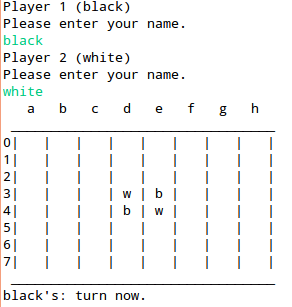
\includegraphics[width=2.5in]{screen2}
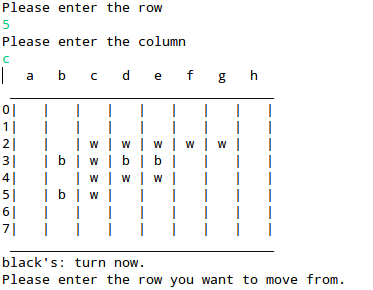
\includegraphics[width=3in]{screen1}

\end{document}
